% Created 2013-03-20 Wed 13:53
\documentclass[11pt,presentation]{beamer}
\usepackage[utf8]{inputenc}
\usepackage[T1]{fontenc}
\usepackage{fixltx2e}
\usepackage{graphicx}
\usepackage{longtable}
\usepackage{float}
\usepackage{wrapfig}
\usepackage{soul}
\usepackage{textcomp}
\usepackage{marvosym}
\usepackage[nointegrals]{wasysym}
\usepackage{latexsym}
\usepackage{amssymb}
\usepackage{hyperref}
\tolerance=1000
\AtBeginSection[]{\begin{frame}<beamer>\frametitle{Topic}\tableofcontents[currentsection]\end{frame}}
\providecommand{\alert}[1]{\textbf{#1}}

\title{大数据环境下信息抽取模板自动发现与聚类}
\author{计92 丘骏鹏 2009011282}
\date{指导老师:朱小燕~郝宇}
\hypersetup{
  pdfkeywords={},
  pdfsubject={},
  pdfcreator={Emacs Org-mode version 7.8.11}}

\usetheme{Singapore}\usecolortheme{crane}
\usepackage{listings}\usepackage{fontspec}\usepackage{xunicode}\usepackage{xltxtra}\usepackage{xeCJK}\beamerdefaultoverlayspecification{}
\setmainfont{Times New Roman}\setmonofont{Courier New}\setCJKmainfont[BoldFont=YouYuan]{SimSun}\setCJKfamilyfont{song}{SimSun}\setCJKfamilyfont{msyh}{微软雅黑}\setCJKfamilyfont{fs}{FangSong}
\setbeamertemplate{bibliography item}[text]
\begin{document}

\maketitle

\begin{frame}
\frametitle{Outline}
\setcounter{tocdepth}{3}
\tableofcontents
\end{frame}


\section{Introduction}
\label{sec-1}
\begin{frame}
\frametitle{Background}
\label{sec-1-1}

\begin{itemize}
\item 已经获取到海量的新闻、博客、论坛等网页原始数据,需要从中提取结构化的信息
\item 从已有数据中抽取模板,利用模板去抽取相似网页中的信息
\item 新的网页可能采取新的模板,需要自动检测,分类和抽取这些新的模板
\end{itemize}
\end{frame}
\begin{frame}
\frametitle{Motivation}
\label{sec-1-2}

\begin{itemize}
\item 一个网站可能采用多个模板,如果采用人工标注模板的办法工作量很大
\item 前期同学的工作主要基于一个网页检测其中的模板,没有利用大数据的优势
\item 充分利用数据的冗余性来进行模板的抽取
\end{itemize}
\end{frame}
\begin{frame}
\frametitle{Related Work}
\label{sec-1-3}
\begin{itemize}

\item 计算HTML文档结构相似度
\label{sec-1-3-1}%
\begin{itemize}
\item 基于DOM Tree本身的方法:Tree Edit Distance\cite{1}。特点:直接对树结构进行操作,算法
     复杂度大,不适用于大量数据的处理。
\item 基于Path集合:每个节点的路径是根节点到该节点的序列,将DOM Tree用路径集合表示,在两个
     网页的路径集合上计算相似度\cite{4,5,6}。
\item 基于Tag集合或序列:直接计算两个网页的Tag集合的Jaccard相似度,或者利用树的遍历将DOM
     Tree转化为Tag序列,然后通过最长公共子序列等方法计算相似度\cite{4,5,8}。
\item 基于傅里叶变换:将文档结构转化为一个序列,将其视为时序序列,用傅里叶变换变换
     到频域计算幅度差别\cite{4,7}。
\end{itemize}

\end{itemize} % ends low level
\end{frame}
\begin{frame}
\frametitle{Related Work}
\label{sec-1-4}
\begin{itemize}

\item 网页聚类算法
\label{sec-1-4-1}%
\begin{itemize}
\item 基于划分的聚类。主要用的是k-medoids,但需要已知模板个数,对于本问题不太适用。
\item 层次聚类。这种聚类算法不需要预先知道类的个数,速度较快。
\end{itemize}


\item 模板提取算法
\label{sec-1-4-2}%
\begin{itemize}
\item 无监督方法:利用网页结构和内容的重复出现发现模板,后期需要人工指定语义\cite{2}。
\item 半监督方法:利用少量标注,进行学习,然后抽取出模板。学习过程可以考虑语义的信息\cite{3}。
\end{itemize}

\end{itemize} % ends low level
\end{frame}
\section{Idea \& Design}
\label{sec-2}
\begin{frame}
\frametitle{Idea}
\label{sec-2-1}

\begin{itemize}
\item 实验的数据量决定了设计的算法不能太复杂,但同时数据的冗余也可以弥补算法的粗糙性,
  从而也能获得较好的效果。
\item 每一步可以先采用一些复杂度较低的算法,评价其运行效果和时间,然后再进行改进
\item 同时需要考虑可以动态增加模板和进行并行化处理
\end{itemize}
\end{frame}
\begin{frame}
\frametitle{Framework}
\label{sec-2-2}
\begin{columns}[t]
\begin{column}{0.3\textwidth}
%% \textbf{:BMCOL:B\_ignoreheading:}
\label{sec-2-2-1}

整体框架示意图
\end{column}
\begin{column}{0.7\textwidth}
%% \textbf{:B\_ignoreheading:BMCOL:}
\label{sec-2-2-2}

    \begin{figure}[htb]
    \centering
    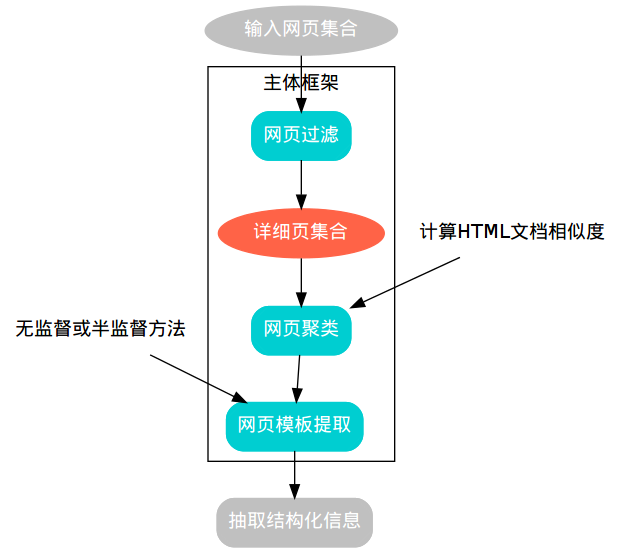
\includegraphics[width=20em,angle=0]{./framework.png}
    \caption{\label{fig:1}framework}
    \end{figure}
\end{column}
\end{columns}
\end{frame}
\begin{frame}
\frametitle{Design}
\label{sec-2-3}
\begin{itemize}

\item 网页过滤
\label{sec-2-3-1}%
\begin{itemize}
\item 网页中含有目录页和详细页,需要过滤掉目录页
\item 要能快速进行计算,不需要过于复杂的机器学习算法
\item 可以采用URL特征结合一些文本特征,比如目录页一般是一些超链接列表,且一般都
      是短文本
\end{itemize}

\item 聚类
\label{sec-2-3-2}%
\begin{itemize}
\item 计算相似度可以采用基于Path集合或者Tag集合的方法,并可以利用一些已有的集合
       相似度的近似算法,降低计算复杂度
\item 采用层次聚类方法进行模板的自动聚类
\item 初步计划参照\cite{4,5,6}的方法进行实现
\end{itemize}
\end{itemize} % ends low level
\end{frame}
\begin{frame}[fragile]
\frametitle{模板表示}
\label{sec-2-4}
\begin{itemize}

\item DOM Tree
\label{sec-2-4-1}%
\begin{figure}[htb]
    \centering
    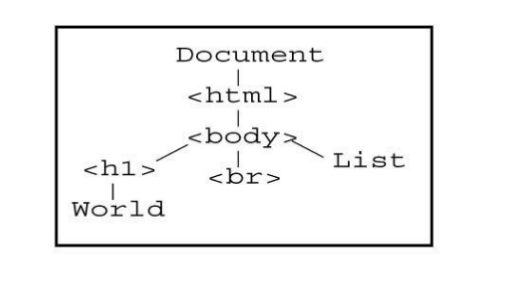
\includegraphics[width=10em,angle=0]{./Selection_001.png}
    \end{figure}

\item Path集合\\
\label{sec-2-4-2}%
\tiny

\begin{verbatim}
| Document\<html>                   |
| Document\<html>\<body>            |
| Document\<html>\<body>\<h1>       |
| Document\<html>\<body>\<h1>\World |
| Document\<html>\<body>\<br>       |
| Document\<html>\<body>\List       |
\end{verbatim}
\normalsize

\item Tag序列\\
\label{sec-2-4-3}%
\tiny

\begin{verbatim}
Document,<html>,<body>,<h1>,World,<br>,<List>
\end{verbatim}
\end{itemize} % ends low level
\end{frame}
\begin{frame}
\frametitle{相似度计算}
\label{sec-2-5}
\begin{itemize}

\item 基于Path集合
\label{sec-2-5-1}%
\begin{itemize}
\item Common Path
\end{itemize}
\[
d_{CP}(D_1,D_2)=1-\frac{|p(D_1)\cap p(D_2)|}{\max (|p(D_1)|, |p(D_2)|)}
\]
\begin{itemize}
\item Common Path Shingles
\end{itemize}
\[
d_{CPS}(D_1,D_2)=1-\frac{|S(D_1,w)\cap S(D_2,w)|}{\max (|S(D_1,w)|, |S(D_2,w)|)}
\]
\begin{itemize}
\item MDL\cite{6}\\
利用路径-文档矩阵进行计算,较为复杂,根据实验效果决定是否使用
\end{itemize}
\end{itemize} % ends low level
\end{frame}
\begin{frame}
\frametitle{相似度计算}
\label{sec-2-6}
\begin{itemize}

\item 基于Tag序列
\label{sec-2-6-1}%
\begin{itemize}
\item Tag Vector
\end{itemize}
\[
d_{TV}(D_1,D_2)=\sqrt{\sum_{i=1}^N(v_i(D_1)-v_i(D_2))^2}
\]
\begin{itemize}
\item Longest Common Tag Subsequence
\end{itemize}
\[
d_{LCTS}(D_1,D_2)=1-\frac{|lcts(D_1,D_2)|}{\max(|D_1|,|D_2|)}
\]
\end{itemize} % ends low level
\end{frame}
\begin{frame}
\frametitle{Design}
\label{sec-2-7}
\begin{itemize}

\item 模板抽取
\label{sec-2-7-1}%
\begin{itemize}
\item 可以考虑直接利用聚类的结果(例如,一个类中的文档之间的共同路径集合),利用
      路径集合可以直接表示文档的模板结构
\item 或者采取一些标注,结合一些已有的模板检测算法进行模板的抽取
\end{itemize}

\item 优化和改进
\label{sec-2-7-2}%
\begin{itemize}
\item 在计算相似度时加入其他特征,和结构特征共同考虑。内容特征,比如文本的行间分
      布,tag的属性值,比如某些div的id,CSS类名
\item 考虑算法的并行性,部署到Hadoop集群上,加快算法运行速度
\end{itemize}
\end{itemize} % ends low level
\end{frame}
\section{Schedule}
\label{sec-3}
\begin{frame}
\frametitle{日程安排}
\label{sec-3-1}

\begin{itemize}
\item 1-4周:任务分析,文献阅读,研究算法
\item 5-8周:网页过滤,网页聚类和网页模板提取模块初步实现
\item 9-12周:算法修正,系统改进,结果分析
\begin{itemize}
\item 是否需要改进相似度算法(包括加入新的特征,改变计算方法)
\item 如何设计并行化计算
\item 如何有效评价系统的功能
\end{itemize}
\item 13-15周:论文撰写
\end{itemize}
\end{frame}
\section{References}
\label{sec-4}
\begin{frame}[allowframebreaks]
\frametitle{参考文献}
\label{sec-4-1}

\scriptsize
\bibliographystyle{plain}
\bibliography{proposal}
\end{frame}

\end{document}